\section{Neighbor Discovery Protocol}
\label{sec:technique}
 
Co-residence detection for lambdas must be quick, as lambdas are ephemeral by
nature. As noted earlier, co-residence detection is faster when co-residing
instances on each server communicate among themselves and discover each other.
Assuming that the instances have unique IDs, co-resided instances can exchange
integer IDs with each other using the memory bus channel as a transmission
medium, which allows us to scale co-residency detection.  In this section, we
present a communication protocol that the co-resided instances can use to
achieve communication in a fast and reliable way. We first discuss the
challenges we faced in making the channel reliable before examining the protocol
itself.

\begin{algorithm}[!t]
\caption{Writing 1-bit from the sender}
\label{alg:sender}
\begin{algorithmic}
\STATE $now \leftarrow  time.now()$
\STATE $end \leftarrow now + sampling\_duration$
\STATE $address \leftarrow cache\_line\_boundary-2$
\WHILE{$now < end$}
    \STATE $\_\_ATOMIC\_FETCH\_ADD(address)$
    \STATE $now \leftarrow  time.now()$
\ENDWHILE
\end{algorithmic}
\end{algorithm}

\subsection{Reliable Transmission}
First, we must determine how to reliably transmit information between the sender
and receiver. Senders and receivers can accurately communicate 0-bits and 1-bits
by causing contention on the memory bus. Consider the simple scenario where
there is one sender and one receiver instance on a machine, and the sender has a
set of bits that it needs to communicate with the receiver via the memory bus
covert channel.  To communicate a 1-bit, the sender instance causes contention
on the memory bus by locking it using the special memory locking operations
(discussed in section~\ref{sec:background:membus}). The receiver would then
sample the memory bus for contention, inferring whether the communication is a
1-bit (when contention is observed) or a 0-bit (when contention is not
observed). Pseudo-code for the sender instance is shown in
Algorithm~\ref{alg:sender}.

\subsubsection{Sensing contention} 
Next, we determine how best for the receivers to sense contention on the memory
bus. There are two ways to acheive this. When the memory bus is locked, any
non-cached memory accesses will queue and therefore see higher latencies.  The
receiver can then continually make un-cached memory accesses (referred to as the
\textit{memory probing} receiver in previous literature~\cite{varadarajan2015})
and observe a spike in their latencies to detect contention. On the other hand,
the receiver can also detect memory bus contention by using the same memory
locking operations as the sender (referred to as \textit{memory locking}
receiver) to probe the memory bus. Since only one processor core can lock the
memory bus at a given time, any other concurrent locking operation will see
higher latency. 

Of these two methods, we decide to use the memory locking receiver for our
experiments.  Previous studies~\cite{wuusenix2012,varadarajan2015} have
established that both memory probing and memory locking receivers experience
significant latency overhead during memory bus contention, making them both
viable avenues for sensing the covert-channel. Memory probing involves regular
(un-cached) memory accesses, which is universal, unlike the locking operations
which are rarely used, if at all, by standard applications. This makes memory
probing the only viable option for \textbf{non-cooperative} co-residence
detection, where receivers are not under the senders's control and cannot be
assumed to perform locking operations.  Furthermore, memory probing can be done
on multiple receivers constantly without affecting each other (due to the high
memory bandwidth), which prevents noise in measurements. This is an important
attribute, as memory locking receivers must contend with this noise. However,
bypassing multi-levels of caches in today's servers to perform memory accesses
with reliable consistency is a challenging task. Even with a reliable
cache-bypassing technique, the variety of cache architectures and sizes that we
encounter on different clouds would make tuning the technique to suit these
architectures an arduous task while reducing the applicability of our overall
co-residence detection mechanism. 
%Thus, we decide to use the memory locking receiver as our sensing mechanism.
%% we already said it at the beginning of the paragraph


\begin{algorithm}[!t]
\caption{Reading a bit in the receiver}
\label{alg:receiver}
\begin{algorithmic}[1]
\STATE $now \leftarrow  time.now()$
\STATE $end \leftarrow now + sampling\_duration$
\STATE $sampling\_rate \leftarrow num\_samples / sampling\_duration$
\STATE $address \leftarrow cache\_line\_boundary-2$
\STATE $samples \leftarrow \{\} $
\WHILE{$now < end$}
    \STATE $before \leftarrow RDTSC()$
    \STATE $\_\_ATOMIC\_FETCH\_ADD(address)$
    \STATE $after \leftarrow RDTSC()$
    \STATE $samples \leftarrow samples \cup \{(after-before)\}$
    \STATE \textbf{wait until} $NEXT\_POISSON(sampling\_rate)$
    \STATE $now \leftarrow  time.now()$
\ENDWHILE
\STATE $ks\_val \leftarrow KOLMOGOROV\_SMIRINOV(samples, baseline)$
\STATE \textbf{return} $ks\_val < ksvalue\_threshold$
\end{algorithmic}
\end{algorithm}


\subsubsection{Sampling frequency}
Another challenge for our protocol is determining an adequate sampling
frequency. Ideally, a memory locking receiver would loop locking operations and
determine contention in real-time by identifying a decrease in the moving
average of the number of operations. Note that, in this case, there is
essentially no difference between the sender and receiver (i.e., both
continually issue locking operations) except that the receiver is taking
measurements. This is adequate when there is a single sender and
receiver~\cite{varadarajan2015}, but when there are multiple receivers, the mere
act of sensing the channel by one receiver causes contention and other receivers
cannot differentiate between a silent (0-bit) and a locking (1-bit) sender. To
avoid this, we space the sampling of memory bus such that no two receivers would
sample the bus at the same time, with high probability. We achieve this by
using large intervals between successive samples and a poisson-sampling to
prevent time-locking of receivers. We determined that a millisecond poisson gap
between samples is reasonable to minimize noise due to collisions in receiver
sampling~\ref{fig:membus_clouds}, assuming ten co-resided receivers and a few
microsecond sampling time.

\subsubsection{Sample Size} 
\label{sec:method:samplingdur}
In addition to adequate sampling frequency, we must also determine sample size.  
A receiver can confirm contention with high confidence with only a
few samples, assuming that the sender is actively causing contention on the
memory bus and the receiver is constantly sampling the memory bus throughout the
sampling duration. However, in practice, the time-sharing of processors
produces difficulties. The sender is not continually causing contention, and
neither is the receiver sensing it, as they are context-switched by the
scheduler, which runs other processes. Assuming that the sender and receiver are
running on different cores, the amount of time they are actively communicating
depends on the proportion of time they are allocated on each core and how they
are scheduled. 

To illustrate such behavior, we run a sender-receiver pair using
lambdas~\cite{awslambda} of various sizes on AWS, and compare the distribution
of latencies seen by the receiver during the contention in each case.
Figure~\ref{fig:context_switching} shows that the much smaller 128 MB lambdas
(which probably share a CPU core and are thus context-switched) exhibit less
active communication than the bigger 3 GB lambdas (which may run on dedicated
cores). This means that smaller instances that tend to share processor cores
with many other instances may need to pause for more time and collect more
samples to make up for lost communication due to scheduling.
% Since the typical scheduling quantum is on the order of milliseconds, they 
% will need at least a second?


\begin{figure}[!t]
  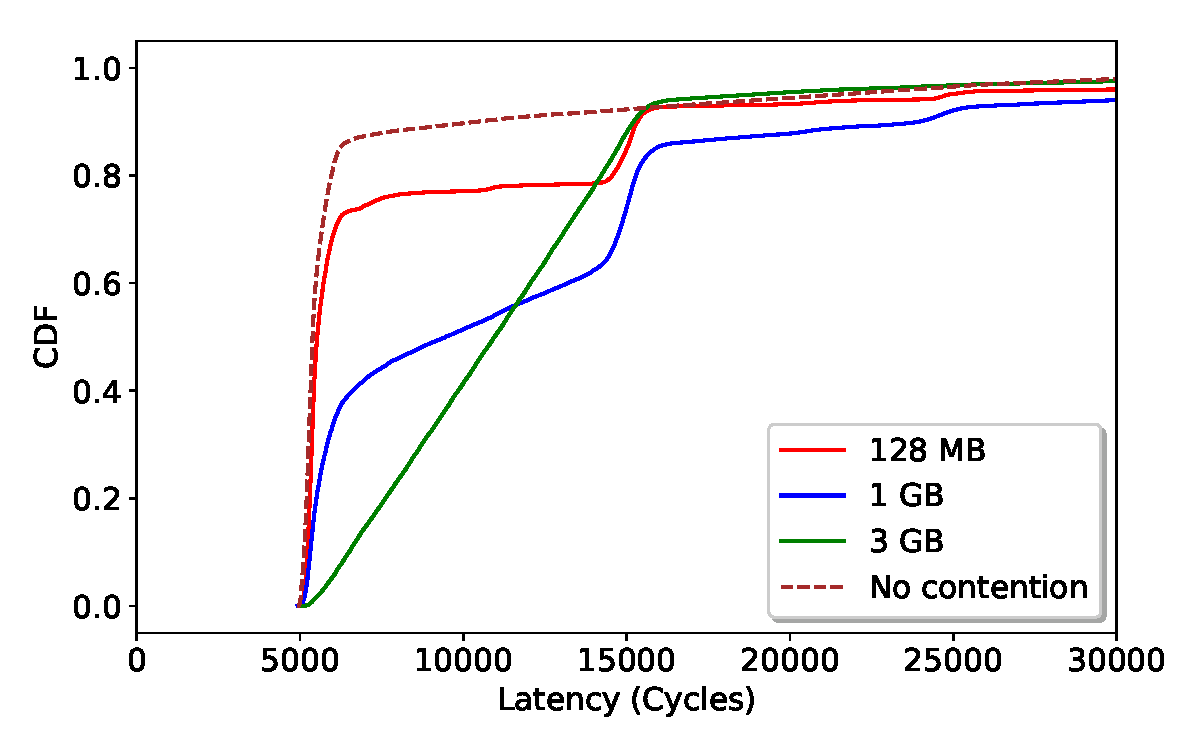
\includegraphics[width=.99\linewidth]{fig/lambda_sched_effect.pdf}
  \caption{We present a CDF of latencies observed by 128 MB, 1 GB and 3 GB
  Lambdas during contention. The 128 MB lambda pair sees less contention due to
  more context switching, whereas the 1 GB and 3 GB lambdas see progressively
  more contention compared to the baseline, which we attribute to their relative
  stability on the underlying physical cores. 
\label{fig:context_switching}}
\end{figure}

\subsubsection{Overcoming noise} 
\label{sec:method:noise}
Along with context switching and sensing noise, there are other imperfections in
the measurement apparatus that may cause noise. For example, we use the
difference in readings from the timestamp counter of the processor (RDTSC)
before and after the locking operation to measure the latency of the operation
in cycles. If the receiver process is context-switched in between the timer
readings (e.g., at line eight in Algorithm~\ref{alg:receiver}), the latency
measured from their difference will be orders of magnitude higher as it includes
the waiting time of the receiver process in the scheduler queue - which we
believe is what contributes to the long tail in
Figure~\ref{fig:context_switching}. To overcome missed samples and noise, we
record hundreds of samples and compare it to the baseline distribution of
latencies sampled without contention. We then need to compare and differentiate
the observed sample of latencies from the baseline to establish contention. To
do this, we use a variant of the two-sample Kolomogorov-Smirinov (KS) test,
which typically compares the maximum of the absolute difference between
empirical CDFs of samples (in our variant, we take the \emph{mean} of the
absolute difference instead of the maximum\amirian{do we know why?}). Using this
measure, we can categorize a KS-value above a certain threshold as a 1-bit
(contention) and a value below the threshold as 0-bit (baseline).

To determine the KS-threshold, we deploy a large number of lambdas across AWS
regions. Some of these lambdas cause contention (aka senders) while others
observe contention by collecting samples of latencies (aka receivers). Each of
the samples may or may not have observed contention depending on whether the
receiver was co-resided with a sender lambda (an unknown at this point). We then
calculate the KS-value for each sample against the baseline and plot a CDF of
these values for lambdas of different sizes in Figure~\ref{fig:ks_values}.
Ideally, we expect a bimodal distribution (stepped CDF) with the upper and
lower peaks corresponding to samples that have and have not seen contention, and
a big gap between the two (long step). Fortunately, we observe this
differentiation with larger lambda sizes (which allows us to choose a clear
threshold), but we do not observe a clear differentiation with smaller lambdas,
where scheduling instability causes lossy communication (discussed
in~\ref{sec:method:samplingdur}).  This trend also reflects in the reliability
of our technique across various lambda sizes, as we will show in our evaluation.
Based on the plot, we picked a KS-threshold at 3.0 which seems to be consistent
across AWS regions, suggesting that this threshold is a platform constant.

We present the pseudo-code of a receiver lambda in Algorithm~\ref{alg:receiver},
which includes all the challenges and subsequent solutions discussed thus
far.

\subsubsection{Clock synchronization} 
Since communicating each bit of information takes time (i.e., receiver sampling
duration), our algorithm requires synchronizing the sender and receiver at the start
of each bit. In traditional analog channels, this is achieved either using a
separate clock signal or a self-clocking signal encoding. For example, prior
work~\cite{whispers} uses differential Manchester encoding for clock
synchronization for the memory bus covert channel. Using self-clocking encodings
becomes more challenging when there are multiple senders and receivers. In this
work, we use the system clock for synchronizing communication.  All the
instances involved in the communication are executing on the same physical
server and share the server's clock. On AWS, for example, we observe that the
system clock on lambdas is precise up to nanoseconds. 
Assuming that clocks between different lambdas only exhibit a drift in the order
of microseconds, sampling at a millisecond scale should provide us a margin for
synchronization mismatch. Since we do not observe any synchronization-related
noise in our results, we believe this is a reasonable assumption.


\begin{figure}[!t]
  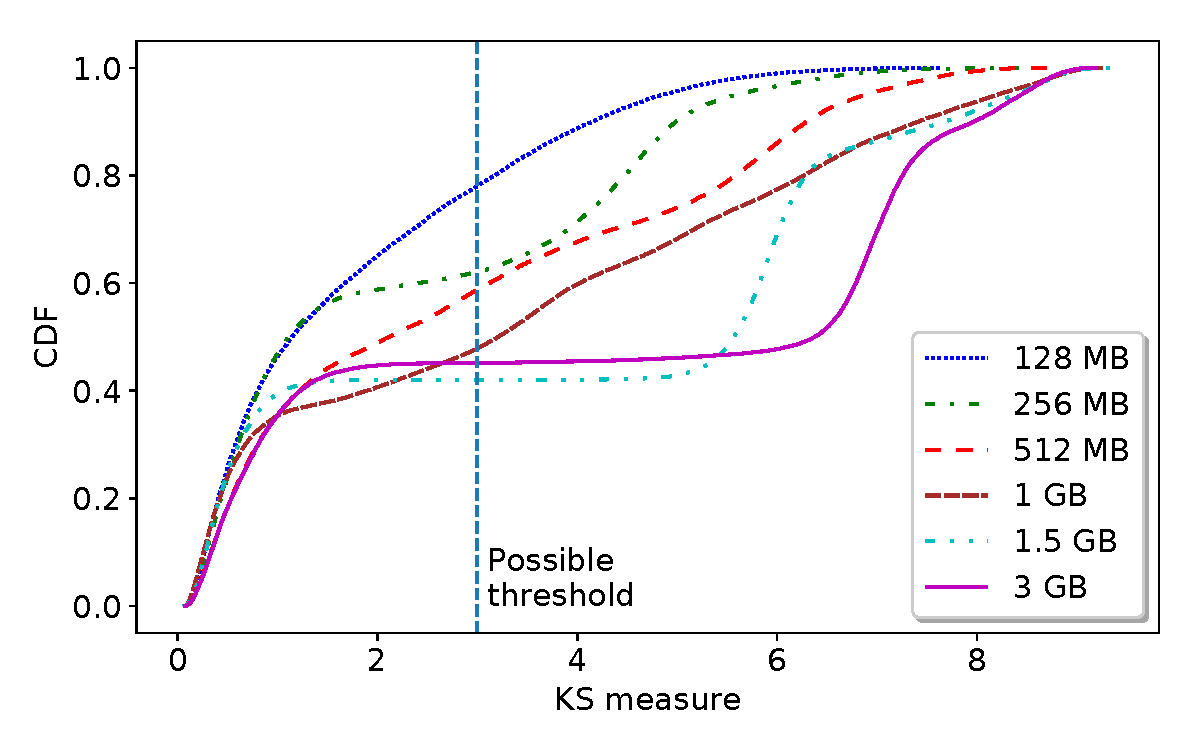
\includegraphics[width=.99\linewidth]{fig/ksvalues.pdf}
  \caption{We present a CDF of KS values observed for various lambda sizes. A bimodal distribution 
  with a longer step allows us to pick a KS-threshold that enables our technique to differentiate 
  between 0-bit and 1-bit with high confidence. 
\label{fig:ks_values}}
\end{figure}

\subsubsection{Handling Collisions}
In the preceeding section, we discussed using a communication channel with
synchronized time slots. In each time slot, an instance can reliably send
(broadcast) or receive (listen) a bit by causing or sensing for contention.
Given that there are multiple instances that may want to broadcast information
on the channel, we must next determine which instance broadcasts first, to avoid
collisions. Traditional channels like Ethernet or Wireless detect and avoid
collisions by employing a random exponential backoff mechanism.  Such a
mechanism will be challenging to implement in our channel for two
reasons. First, lambda instances do not have the capability of sensing the
channel while sending a bit, which is required for detecting collisions;
instances can either cause contention or sense it, but not both. Note that
senders do experience a higher latency for locking operations when other senders
are simultaneously causing contention. However, reliably judging this higher
latency requires each sender to already have calculated a baseline of latencies
without collisions%, which returns this discussion to the original problem of avoiding collisions.  
Second, even implementing a random or exponential backoff mechanism
will introduce significant overhead before any meaningful communication occurs.
This overhead will also increase as the number of instances involved increases.
Since each time slot could take up to 1 second, this additional overhead can
make the whole communication very slow. We address this by designing a 
specialized communication protocol that allows for collisions but conversely is
less expressive, as we will see in the next section.



\subsection{Protocol}
\label{sec:protocol}


\begin{algorithm}[!t]
\caption{ID exchange protocol \todo{Improve pseudo-code}}
\label{alg:protcol}
\begin{algorithmic}[1]
\STATE $sync\_point \leftarrow$ {Start time for all instances}
\STATE $ID \leftarrow$ {Instance ID}
\STATE $N \leftarrow$ {Number of bits in ID}
\STATE $advertising \leftarrow TRUE$
\STATE $instances \leftarrow \{\} $
\STATE $WAIT\_TILL(sync\_point)$
\WHILE{$id\_read$}
    \STATE $slots \leftarrow 0$
    \STATE $id\_read \leftarrow 0$
    \STATE $participating \leftarrow advertising$
    \WHILE{$slots < N$}
        \STATE $bit \leftarrow$ {$slots^{th}$ most significant bit of ID}
        \IF{$participating$ \textbf{and} $bit$}
            \STATE $WRITE\_BIT()$               (Alg. \ref{alg:sender})
            \STATE $bit\_read \leftarrow 1$
        \ELSE
            \STATE $bit\_read \leftarrow READ\_BIT()$       (Alg. \ref{alg:receiver})
            \IF{$bit\_read$}
                \STATE $participating \leftarrow FALSE$
            \ENDIF
        \ENDIF
        \STATE $id\_read \leftarrow 2 * id\_read + bit\_read$
        \STATE $slots \leftarrow slots + 1$
    \ENDWHILE
    \IF{$id\_read = ID$}
        \STATE $advertising \leftarrow FALSE$
    \ENDIF
    \STATE $instances \leftarrow instances \cup \{id\_read\}$
\ENDWHILE
\STATE \textbf{return} $instances$
\end{algorithmic}
\end{algorithm}

When considering a communication channel for lambda co-residence detection, we
note that the channel need not be general and expressive as lambdas only need to
communicate their IDs with one another. Thus, we assume that each instance
involved has a unique fixed-length (say \emph{N}) bit-string corresponding to
its ID that must be communicated.  As such, we propose a communication protocol
that exchanges these bit-strings while allowing for collisions. We divide the
running time of the protocol into phases, with each phase executing for an
interval of \textit{N} bit-slots. Each phase has a set of participating
instances, which in the first phase would be all of the co-resided instances. In
each bit-slot \textit{K} of \textit{N} slots in a phase, every participating
instance broadcasts a bit if the $K^{th}$ bit of its bit-string (ID) is 1,
otherwise it listens for a 0 or 1. If an instance senses a 1 while listening, it
stops participating, and listens for the rest of the phase. Thus, only the
instances with the highest ID among the initial set of participating lambdas
continues broadcasting until the end of the protocol, effectively advertising
its full ID to the rest of the (now listening) lambdas. In the next cycle, the
lambda with the previously highest ID now only listens, allowing the next
highest instance to advertise its ID, and so on.  Since the IDs are unique,
there will always be only one instance that broadcasts in every phase. The
protocol ends after \textit{x} phases (where \textit{x} is number of co-resided
instances), when none of the instances broadcast for \textit{N} consecutive
bit-slots. The pseudo-code of the protocol is provided in Algorithm
\ref{alg:protcol}. Note that the protocol itself is channel-agnostic and can be
extended for other (future) covert channels with similar channel properties.

% Figure moved here for formatting
\begin{figure}[!t]
  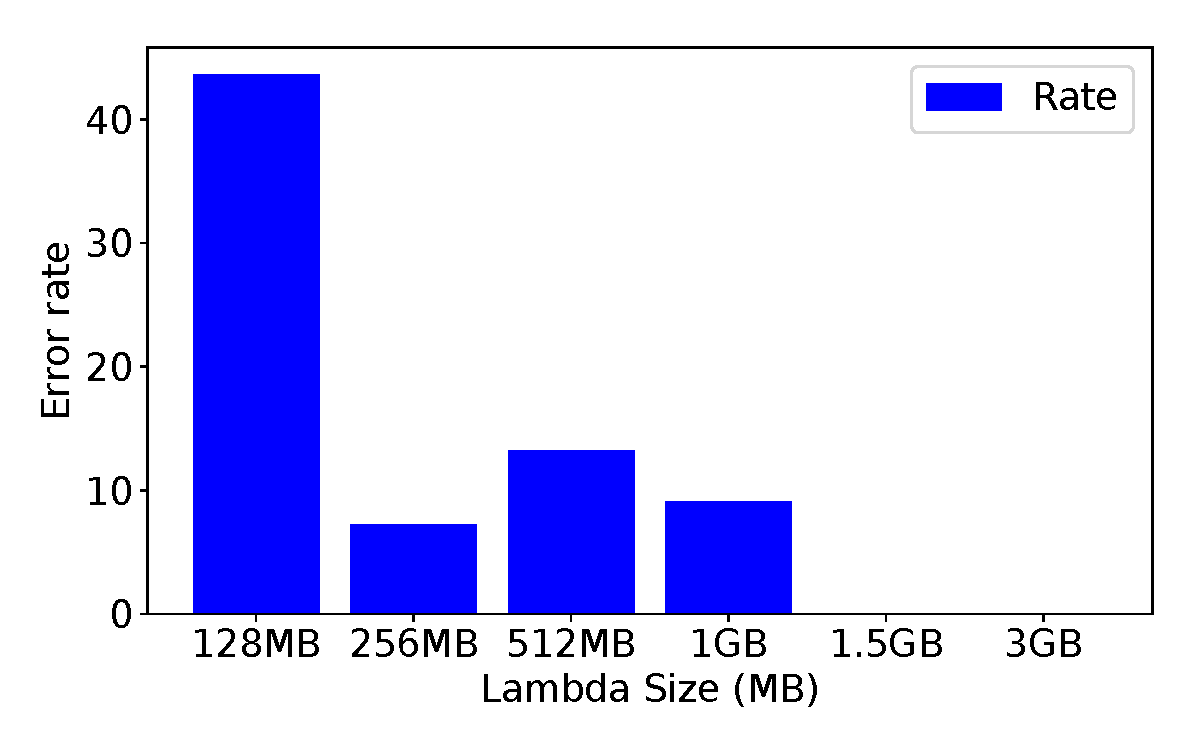
\includegraphics[width=.99\linewidth]{fig/errorrates.pdf}
  \caption{This figure presents the error rate (as a fraction of 1000 lambdas
  deployed) for different lambda sizes in the AWS Middle-East region. 
\label{fig:errorrates}}
\end{figure}

\subsubsection{Time Complexity}
\label{sec:protocol:complexity}
Assuming \textit{N} total deployed instances to the cloud, the bit-string needs
to be $\log_2N$ bits to uniquely identify each instance. If a maximum \textit{K}
of those instances are launched on the same server, the protocol executes for
\textit{K} phases of $\log_2N$ bit-slots each, taking $(K+1)*\log_2N$ bit-slots
for the whole operation. For example, assuming 10,000 deployed lambdas and a
maximum of 10 co-resided instances on each server, the entire  co-residence
detection requires around four minutes to fully execute (with 1-second time
slots). In fact, it is not necessary to run the protocol for all \textit{K}
phases. After the first phase, all the co-resided instances would know one of
their neighbors (as each phase reveals the ID of the biggest participating
instance to others).  If we use IDs that are globally unique, all the
co-resided instances will see the same ID. The instances can then exchange these IDs
offline (e.g., through the network) to infer the rest of their neighbors. This
simplification removes the dependency on number of co-resided instances
(\textit{K}) and decreases the complexity to $O(\log_2N)$, allowing the entire
protocol to finish within a minute instead of four.


% \subsubsection{Limitations}
% challenge with same core scheduling. - write a list of drawbacks?
% this could be overcome by getting 
% redundant info and constructing 
% the graph
